\documentclass[apaper4,12p]{scrartcl}
\usepackage[ngerman]{babel}
\usepackage[utf8]{inputenc}
\usepackage[T1]{fontenc}
\usepackage{csquotes}
\usepackage{graphicx}
\usepackage{dirtree}
\usepackage{svg}
\usepackage{amsmath}
\renewcommand{\figurename}{Abbildung}
\setcounter{secnumdepth}{4}
\setcounter{tocdepth} {2}
\setcounter{secnumdepth} {3}
\usepackage{marvosym}
\usepackage{fancyhdr}
\pagestyle{fancy}
\renewcommand{\sectionmark}[1]{\markright{\thesection\ #1}}
\fancyhf{} % supprime les en-t\^etes et pieds pr\'ed\'efinis
\fancyhead[LE,RO]{\bfseries\thepage}% Left Even, Right Odd
\fancyhead[LO]{\bfseries\rightmark} % Left Odd
\fancyhead[RE]{\bfseries\leftmark} % Right Even
\renewcommand{\headrulewidth}{0.5pt}% filet en haut de page
\addtolength{\headheight}{0.5pt} % espace pour le filet
\renewcommand{\footrulewidth}{0pt} % pas de filet en bas
\fancypagestyle{plain}{ % pages de tetes de chapitre
	\fancyhead{} % supprime l'entete
	\renewcommand{\headrulewidth}{0pt} % et le filet
	\fancyfoot[C]{\bfseries\thepage} %contient uniquement le num de page en pieds de page
}

\usepackage{color}

\definecolor{gris10}{gray}{0.9} %si on veut utiliser une nuance de la couleur grise
\definecolor{bleufonce}{rgb}{0,0,0.55}
\usepackage[top=25mm, bottom=25mm, left=25mm , right=25mm]{geometry}
\linespread{1.2} %interligne
%\setlength{\parindent}{0 pt} %pas d'indentation
\setlength{\parskip}{1.5ex plus 1ex minus 0.5ex}
\addto\captionsfrench{%
	\renewcommand{\listfigurename}{Liste des figures}%
}
\usepackage{listings}


\definecolor{dkgreen}{rgb}{0,0.6,0}
\definecolor{gray}{rgb}{0.5,0.5,0.5}
\definecolor{mauve}{rgb}{0.58,0,0.82}

\lstset{frame=tb,
	language=java,
	aboveskip=3mm,
	belowskip=3mm,
	showstringspaces=false,
	columns=flexible,
	basicstyle={\small\ttfamily},
	numbers=none,
	numberstyle=\tiny\color{gray},
	keywordstyle=\color{blue},
	commentstyle=\color{dkgreen},
	stringstyle=\color{mauve},
	breaklines=true,
	breakatwhitespace=true,
	tabsize=3
}

\definecolor{maroon}{rgb}{0.5,0,0}
\definecolor{darkgreen}{rgb}{0,0.5,0}
\lstdefinelanguage{XML}
{
	basicstyle=\ttfamily,
	morestring=[s]{"}{"},
	morecomment=[s]{?}{?},
	morecomment=[s]{!--}{--},
	commentstyle=\color{darkgreen},
	moredelim=[s][\color{black}]{>}{<},
	moredelim=[s][\color{red}]{\ }{=},
	stringstyle=\color{blue},
	identifierstyle=\color{maroon}
}

\title{Wissenschaftliche-Vertiefung-Ausarbeitung}
\date{01.07.2019} 
\author{Mohamed Karim Swissi  }
\begin{document}
\tableofcontents
\newpage

\section{Motivation}
\section{Einleitung}
\subsection{Aufgabenbeschreibung}

Am Anfang stand die Idee, dass ich mich immer tiefer mit Automatisierung beschäftige. Deshalb fiel die Wahl auf ein Projekt in diese Richtung.
Im Rahmen dieser wissenschaftliche Vertiefung Modul wird ein auf Docker basierendes Testsystem entwickelt.
Dieses Test-Framework soll die studenten helfen, ihre Übungsaufgaben automatisiert zu testen.
\newline
Der Student lädt seinen Quellcode über eine Web-Benutzeroberfläche hoch, dieser Service steht den Studenten nach der Registrierung auf der Testplattform zur Verfügung.Für mich ist die Studenten Registrierung in der Tat eine Erstellung eines eigenen Remote-Testraums, der dadurch der Testprozess verwaltet wird, und das, was ich in dieser Ausarbeitung im Detail erklären werde. Nach Abschluss des Testprozesses erhält der Student einen Bericht mit dem Ergebnis seines Tests. Darüber hinaus sollte dieses Test-Framework der Lehrkraft  die Möglichkeit geben, die individuellen Testaufgaben der Studenten zu kontrollieren.
\subsection{Herangehensweise}
In diesem Abschnitt werde ich die Techniken und Technologien vorstellen, die in diesem Projekt verwendet werden. Daher wurde das Konzept des Code-Testens erläutert. Ebenso wird das in diesem Projekt verwendete Unit-Test-System besprochen. Anschließend werden die Rolle des Jenkins-Tools im Projekt und die Bedeutung dieses Tools für die Automatisierung des Testprozesses erläutert, dann folgt eine ausführliche Erläuterung der Verwendung von Docker im Projekt. Abschließend eine Erläuterung von Git-Hosting und Jgit, die einen der wichtigsten Teile des Projekts darstellen.
\newline
Im Hauptabschnitt wird dann die Erstellung der Testplattform erläutert. Es wird die Architektur beschrieben, und die Entscheidungen, die getroffen wurde, indem die Techniken ausgewählt wurde, mit denen das Projekt die Anforderungen erfüllt. Außerdem werden der Ablauf des Testverfahrens und die internen Prozesse des Bestandteils der Testplattform vorgestellt. Dann werden die Installationsanweisungen und Verzerrungen der Testplattform klarstellen.

\section{Grundlagen}
\subsection{Code Testing}
Beim Softwaretesten wird ein Programm oder eine Anwendung ausgeführt, um die Fehler zu ermitteln und um zu überprüfen, ob die erforderlichen Bedingungen erfüllt sind.
\newline
Softwaretestverfahren können in 2 Gruppen unterteilt werden:Statisches / Statisches Testen.
\subsubsection{Manual testing( Statisches)}
Eine Softwaretesttechnik, bei der die Software getestet wird, ohne den Code auszuführen. Es besteht aus zwei Teilen:
\begin{itemize}
	\item Review - Wird normalerweise verwendet, um Fehler oder Unklarheiten in Dokumenten wie Anforderungen, Design, Testfällen usw. zu finden und zu beseitigen.
	\item Statische Analyse - Der von Entwicklern geschriebene Code wird (normalerweise mithilfe von Werkzeugen) auf strukturelle Fehler analysiert. 
\end{itemize}
\subsubsection{Automated Testing(Dynamisches)}
Beim dynamischen Testen wird die Software auf die Eingabewerte geprüft und die Ausgabewerte analysiert. Es gibt verschiedene Stufen dynamischer Testtechniken: 
\begin{itemize}
	\item Unit Testing
	\item Integration Testing
	\item System Testing
	\item Acceptance Testing
\end{itemize}
In diesem Fall verwenden wir eines Dynamisches Testen, um die Programmieraufgaben der Studenten zu bewerten.
\subsection{Das Unit Testsystem}
\subsection{Jenkins}
\subsubsection{Einführung}
\subsubsection{Jenkins buildflow}
\subsubsection{Jenkins pipeline}
\subsubsection{Jenkins multijob}
\subsubsection{Jenkinsfile}
\subsection{Docker}
\subsubsection{Einführung}
\subsubsection{Docker Architektur}
Nach meiner Erfahrung besteht eine der einfachsten Möglichkeiten, Docker zu verstehen und anzuwenden, darin, sich einen Überblick darüber zu verschaffen, wie die Docker-Plattform im Hintergrund aufgebaut ist.
\newline
\begin{figure}[htp]
	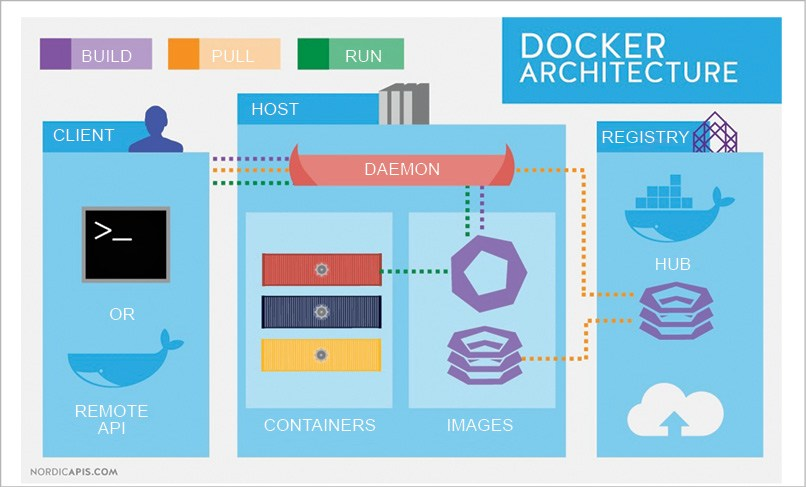
\includegraphics[scale=2]{Figure-1-Docker-container-architecture}
	\caption{Docker Architektur}
	\label{img:grafik-dummy}
\end{figure}
In Abbildung 1 sehen Sie die Hauptkomponenten einer Docker-Installation:
\begin{itemize}
	\item Im Zentrum steht der Docker-Daemon, der für das Erstellen, Ausführen und Überwachen von Containern sowie für das Erstellen und Speichern von Images zuständig ist. Der Docker-Dämon wird vom Host-Betriebssystem verwaltet.
    \item Der Docker-Client befindet sich auf der linken Seite und wird für die Kommunikation mit dem Docker-Daemon über HTTP verwendet. Ein Docker-Client kann mit mehr als einem Daemon kommunizieren, da sich der Docker-Client auf demselben Host wie der Daemon oder über eine Verbindung auf einem Remote-Host befinden kann. Der Docker-Client bietet eine Befehlszeilenschnittstelle (Command Line Interface, CLI), mit der Sie Anwendungsbefehle für einen Docker-Dämon erstellen, ausführen und stoppen können.
    \item Docker-Registrys speichern und verteilen images, die Standardregistrierung heißt Docker Hub und hostet Tausende von öffentlichen Images. Viele Unternehmen führen eigene Register, in denen kommerzielle oder vertrauliche Images gespeichert werden können. Der Docker-Daemon lädt als Reaktion auf Docker-Pull-Requests Images von Registrys herunter. Es werden auch automatisch Images heruntergeladen, die in Docker-Run-Requests und in der FROM-Anweisung von Dockerfiles angegeben sind, wenn sie nicht lokal verfügbar sind.
\end{itemize}
Wenn in diesem Abschnitt etwas nicht verstanden wird, wie z. B. Bilder, Dockerfile ..., machen Sie sich keine Sorgen, da in den folgenden Abschnitten alles im Detail erläutert wird.
\subsubsection{Docker Images}
\subsubsection{Docker Container}
\subsubsection{Docker Volumes}
\subsubsection{Data Container}
\subsubsection{Docker Compose}
\subsubsection{DockerFile}
\subsection{Git-Hosting mit Gogs}
\subsubsection{Einführung}
\subsubsection{Datenbankeinstellung}
\subsubsection{JGit}
\subsubsection{Webhook}
\section{Test-C Plattform}
\subsection{Einführung}
In diesem Abschnitt wird die Test C-Plattform detailliert beschrieben, wobei zunächst die Zusammensetzung der gesamten Programmarchitektur erörtert wird, anhand derer die Programmkomponenten separat diskutiert werden können. Nach der Erklärung der Komponenten des Programms auf separate Weise, wird im Abschnitt (Interne Prozesse) genau erläutert, wie sie zusammenarbeiten.
\newline
Wenn der Leser das oben Genannte versteht, kann er verstehen, was ich im Abschnitt  (Ablauf des Testverfahrens) erläutert wird.
\subsection{Architektur}
\begin{figure}[h!]
	\begin{center}
		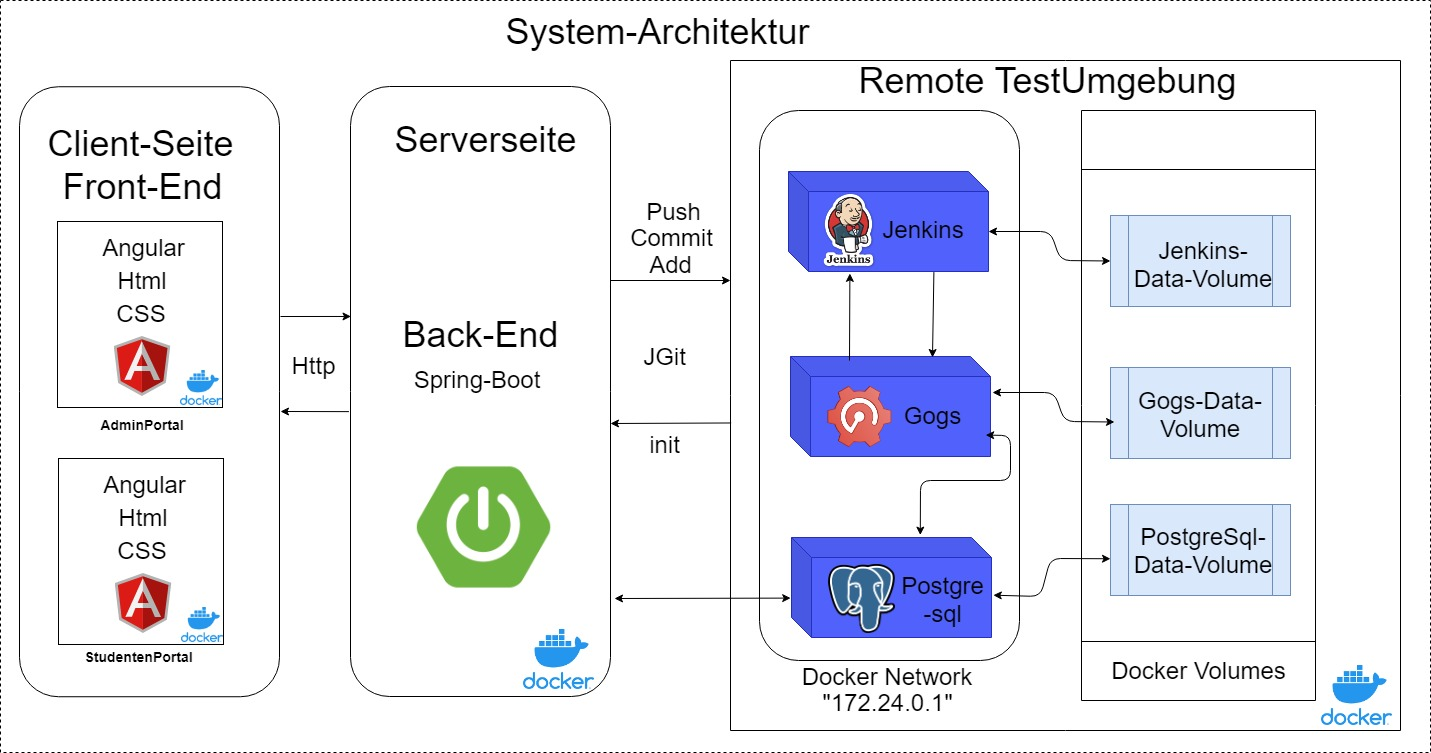
\includegraphics[width=17.5cm, height=13cm]{Test-C-Plattform-Arch.jpg}
		\caption{Architektur Test-C-Plattform } 
		\label{ Architektur Test-C-Plattform } 
	\end{center}
\end{figure}
Wie in der Abbildung 2 gezeigt, ist die Test-C-Plattformarchitektur in drei Hauptteile unterteilt: Client-Seite, Serverseite und Remote-TestUmgebung.
\newline
Die Wahl der Technologien beruhte auf ihrer Modernität und ihrer Verbreitung auf dem Arbeitsmarkt. In Teil eins des Projekts (Client-Seite/Frontend) wurde die folgenden Techniken verwendet : Angular 7, NGX-Bootstrap, Html, Css, im zweiten Teil des Projekts (Serverseite / BackEnd) wurden Maven und Spring Boot, Spring Security und Ldap ... verwendet. Der dritte Teil des Projekts, in dem der Testprozess durch Jenkins abgeschlossen ist.
\newline
Im folgenden Abschnitt werde ich jeden Teil des Architektur separat erklären.
\subsubsection{Client-Seite (Front-End)}
\begin{figure}[h!]
	\begin{center}
		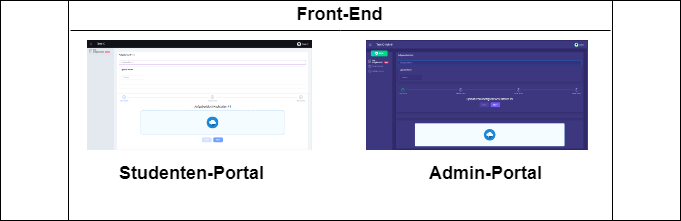
\includegraphics[width=17.5cm, height=7cm]{FrontEnd.png}
		\caption{Front-End } 
		\label{ Front-End } 
	\end{center}
\end{figure}
In diesem Projekt ist die Benutzeroberfläche in zwei Teile unterteilt: das Administrationsportal und das Studentenportal. Beide Portale wurden mit Angular 7, Html, Css und NGX-Bootstrap erstellt.
Über das Administrations Portal kann der Admin Benutzer ein neues Aufgabenblatt erstellen, dies bedeutet, dass ein virtueller Bereich für den Aufgabenblatttest erstellt wird, in dem die Studenten ihre Lösungen für Aufgaben testen können. Der Administrator kann alle Testdateien für jedes Aufgabenblatt in den entsprechenden Testbereich hochladen. Der Administrator kann auch die Testbereiche anzeigen. Jeder Testbereich ist mit dem Namen des zu testenden Aufgabenblatts gekennzeichnet. Für jeden Testbereich werden die spezifischen Testdateien angezeigt und der Administrator kann davon Dateien löschen oder andere hinzufügen.
Über das Studentenportal kann der Student die zu testende Lösungsdatei hochladen und dann an den Testbereich senden, der den Test automatisch durchführt und dem Studenten das Testergebnis anzeigt.
\subsubsection{Remote TestUmgebung}
Die Erklärung dieses Teils des Projekts vor der Erklärung des Mittelteils 'Serverseite' ist eine absichtliche Sache, damit der Leser einfach verstehen kann, was im Back-End passieren wird.
\newline
Die Remote-Testumgebung besteht aus drei miteinander verbundenen Docker-Containern (Jenkins-Container / Gogs-Container / PostgreSql-Container). Jeder Container verfügt über ein eigenes Datenvolumen zum Speichern der Daten. Dadurch wird vermieden, dass Informationen gelöscht werden, wenn der Container ausgeschaltet oder gelöscht wird.
\newline
Um einen Docker-Container in diesem Teil des Projekts zu erstellen, werden zwei verschiedene Methoden verwendet, entweder über eine Dockerfile Datei oder über eine Docker-Compose Datei.
\newline
Für den Jenkins-Container wurde eine Dockerfile Datei verwendet. Der Jenkins-Container besteht hauptsächlich aus einem Jenkins, den Compilern: gcc und g ++, die für den Build verantwortlich sind, und doxygen, das für den Testbericht verantwortlich ist.
\newline
Die Frage, die sich jetzt stellt, ist: Was ist eine Dockerfile Datei?
\newline
Ein Dockerfile ist einfach eine Textdatei mit einer Reihe von Anweisungen (instructions), die genutzt werden können, um ein Docker-Image zu erzeugen.
\newline
\begin{lstlisting}[caption=Dockerfile - jenkins]
FROM jenkins/jenkins

USER root

RUN apt-get -y update && apt-get -y upgrade

# install gcc g++ gfortran
RUN apt-get -y install build-essential

# install static analysis
RUN apt-get -y install doxygen graphviz
\end{lstlisting}
Die FROM-Anweisung legt fest, welches Basisimage zu verwenden ist, wie in diesem Fall Jenkins. RUN-Anweisunggen geben einen Schell-Befehl an, der im Image ausgeführt werden soll. In diesem Fall werden g++, gcc und doxygen ausgeführt.
\newline
Für den Gogs-Container und den PostgreSql-Container wurde eine Docker-Compose Datei verwendet.
Docker Compose wird zum Definieren und Ausführen von Docker-Anwendungen mit mehreren Containern verwendet. Mit Compose wird eine YAML-Datei (docker-compose.yml) verwendet, um die Dienste (services) von der Anwendung zu konfigurieren, wobei jeder Dienst (service) einen Container mit der zum Erstellen erforderlichen Konfiguration darstellt.
\begin{lstlisting}[caption=docker-compose.yml - Gogs/PostgreSql]
version: '2'
services:
app:
image: gogs/gogs:latest
volumes:
- /tmp/gogs-data:/data
ports:
- "3000:3000"
links:
- postgres:postgres
postgres:
image: postgres:alpine
volumes:
- /tmp/gogs-postgres:/var/lib/postgresql/data
environment:
- POSTGRES_USER=postgres
- POSTGRES_PASSWORD=password123
- POSTGRES_DB=gogs
\end{lstlisting}
Gogs ist ein einfacher selbst-gehosteter Git Service, der einfach einzurichten und zu betreiben ist und auf fast allem ausgeführt werden kann. Es ist zu Hundertprozent Open Source unter der MIT OSS-Lizenz. Gogs bietet die Anzeige und Bearbeitung von Repository-Dateien, die Verfolgung von Projektproblemen und ein eingebautes Wiki für die Projektdokumentation.
Gogs benötigt eine Datenbank, um den Quellcode zu speichern, daher wurde hier postgresql ausgewählt.
\newline
Nun stellt sich die Frage, wie die Container miteinander kommunizieren ?
\newline
Damit Docker-Container über den Host-Computer miteinander und mit der Außenwelt kommunizieren können, wird in diesem Fall eine Netzwerkschicht (Docker Networking) eingesetzt. Docker unterstützt verschiedene Arten von Netzwerken, die jeweils für bestimmte Anwendungsfälle geeignet sind: Bridge mode, Host mode, Container mode, und No networking.

\begin{lstlisting}[caption=Docker Network]
[
{
"Name": "gogs-compose_default",
"Id": "e19d76ee7d9f4132329d44e618bea3c5d93466527dd991d35b01fe4262ba6d73",
"Created": "2019-09-09T17:14:13.0772793Z",
"Scope": "local",
"Driver": "bridge",
"EnableIPv6": false,
"IPAM": {
"Driver": "default",
"Options": null,
"Config": [
{
"Subnet": "172.23.0.0/16",
"Gateway": "172.23.0.1"
}
]
},
"Internal": false,
"Attachable": false,
"Ingress": false,
"ConfigFrom": {
"Network": ""
},
"ConfigOnly": false,
"Containers": {
"0e69b0fffaf865665b4c2788f0d43a450301dff06ab1d50fedc4d24c0c97f0b4": {
"Name": "jenkins/jenkins",
"EndpointID": "0fc2f145af6d60b8da71e592299d9a0e2d7f578a392832baa0eb4f9e33b1c6e0",
"MacAddress": "02:42:ac:17:00:04",
"IPv4Address": "172.23.0.4/16",
"IPv6Address": ""
},
"264529e624168c9a64a308f2bbadeb26eb3676e54935de87f42675c114721754": {
"Name": "gogs-compose_app_1",
"EndpointID": "3309a74372ac94794dcf1e6f7df21cda2a54c1b98a608e3a5b9922098831d894",
"MacAddress": "02:42:ac:17:00:03",
"IPv4Address": "172.23.0.3/16",
"IPv6Address": ""
},
"6d04174448af71fd4a5de8735f5ad46e52145f933a3c5fbaa3ea53052eccf168": {
"Name": "gogs-compose_postgres_1",
"EndpointID": "e48d315587aa881a2d77984cb856a446d1c5fb74f6fa2f95bb3be6671b90dba7",
"MacAddress": "02:42:ac:17:00:02",
"IPv4Address": "172.23.0.2/16",
"IPv6Address": ""
}
},
"Options": {},
"Labels": {}
}
]
\end{lstlisting}


\subsubsection{Serverseite (Back-End)}
Nun wird über die Serverseite gesprochen, die für die Kommunikation des Benutzers mit der Testumgebung verantwortlich ist.
\newline
Die Serverseite stellt viele Dienste wie folgt bereit:
\paragraph{Benutzererkennung} In der westfälischen Hochschule Gelsenkirchen basiert die Speicherung der Hauptbenutzeridentitäten auf LDAP-Protokolls (Lightweight Directory Access Protocol) und gespeicherter LDAP-Datenbank. Dies hilft dabei, die Single Sign-On-Technologie (SSO) zu nutzen, die dadurch sich der Benutzer mit derselben ID und denselben Kennwörtern bei allen Anwendungen im selben Netzwerk anmelden kann. Um dies zu erreichen, sind 'spring-boot-starter-security' und 'spring-security-ldap' und 'unboundid-ldapsdk' in diesem Projekt verwendet.

\begin{lstlisting}[language=XML,caption=pom.xml - security dependencies]
<dependency>
<groupId>org.springframework.boot</groupId>
<artifactId>spring-boot-starter-security</artifactId>
</dependency>

<dependency>
<groupId>org.springframework.security</groupId>
<artifactId>spring-security-ldap</artifactId>
</dependency>
<dependency>
<groupId>com.unboundid</groupId>
<artifactId>unboundid-ldapsdk</artifactId>
</dependency>
<dependency>
<groupId>org.springframework.ldap</groupId>
<artifactId>spring-ldap-core</artifactId>
</dependency>
\end{lstlisting}
Unter Verwendung der obigen Abhängigkeiten werden Sicherheitsrichtlinienkonfigurationen wie folgt geschrieben: Zunächst wird festgelegt, welche Dienste der Benutzer ohne Anmeldung bereitstellen kann und bei welchen Diensten er sich anmelden muss. Wenn der Benutzer seinen Benutzernamen und sein Kennwort eingibt, wird überprüft, ob die Authentifikation-Daten gültig sind, indem sie mit den in der LDAP-Datenbank verfügbaren Daten verglichen werden.
\newline
Es wird nun davon ausgegangen, dass der Benutzer gültige Daten eingegeben hat. dh diese Daten sind identisch mit den in der LDAP-Datenbank gespeicherten Daten. Dann wird ein Token generiert und als Antwort auf die Authentifikation-Anfrage zurückgesendet. Dieses Token wird dann vom Frontend verwendet und mit jeder Anfrage gesendet.
\newline
Wird eine Anfrage geschickt, wird vom Backend dann überprüft, ob das Token gültig ist. Ist das der Fall, wird dann die Anfrage an den entsprechenden Controller weitergeleitet und damit die passende Funktion ausgeführt.
\begin{figure}[h!]
	\begin{center}
		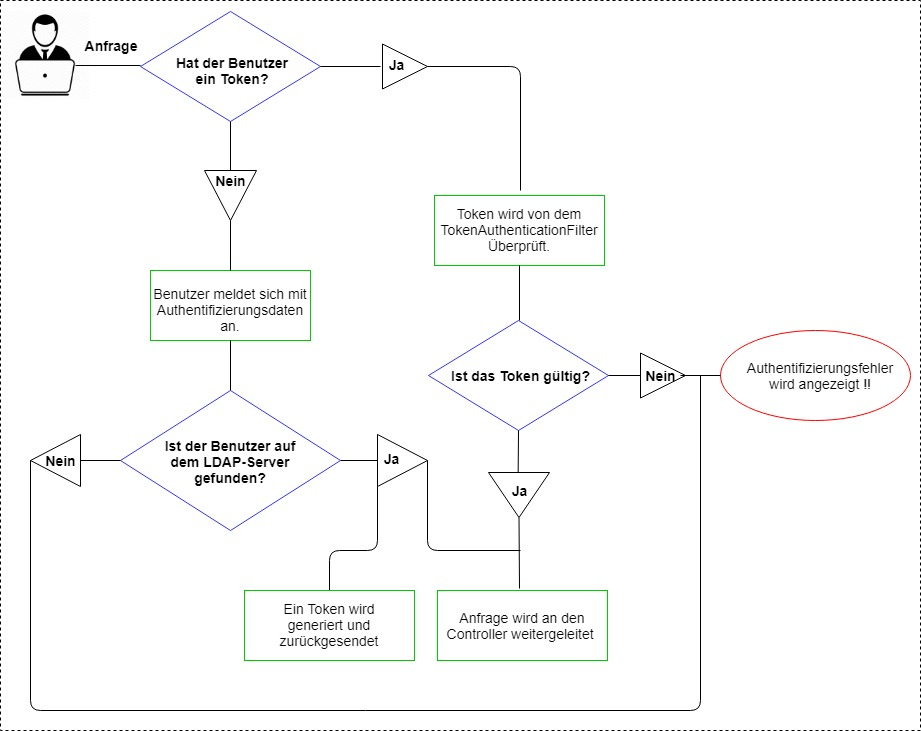
\includegraphics[width=15cm, height=17cm]{Ldap-Auth.jpg}
		\caption{Ldap-Auth } 
		\label{ Ldap-Auth } 
	\end{center}
\end{figure}

\paragraph{Erstellung eines neuen Aufgabenblatts (Admin)}
Wie oben erläutert, ist die Erstellung eines neuen Aufgabenblatts in der Tat eine Einrichtung eines neuen Testbereichs, an dem die Studenten ihre Aufgabenlösungsdateien testen können. Mit anderen Worten, das Erstellen eines neuen Aufgabenblatts hängt vom Erstellen eines neuen Git-Repository ab, das denselben Namen wie das Aufgabenblatt hat. Zum Beispiel (Aufgabenblatt-1) über die Gogs-Oberfläche, die dem Administrator zur Verfügung steht. In diesem Git-Gogs-Repository werden alle zum Testen erforderlichen Dateien gespeichert. Anschließend wird ein Jenkins Multibranch-Pipeline-Job erstellt, der auch denselben Namen wie das Aufgabenblatt hat.
\paragraph{Schaffung von Jenkins Job (Admin)}
Für die Erstellung von Multibranch-Pipeline-Job bietet Jenkins eine REST-API an, die viele Dienste bereitstellt, z. B. das Erstellen und Löschen von Job und viele andere Dinge. Um diese Jenkins-API zu verwenden, muss eine Maven-Abhängigkeit in pom.xml hinzugefügt werden.
\begin{lstlisting}[language=XML,caption=pom.xml - Jenkins-Api]
<dependency>
<groupId>com.offbytwo.jenkins</groupId>
<artifactId>jenkins-client</artifactId>
<version>0.3.7</version>
</dependency>
\end{lstlisting}
Zur Verdeutlichung wird erläutert, wie mit Jenkins-Api einen neuen Job erstellt werden kann. Um einen Job in Jenkins zu erstellen, müssen dem Job  ein Name und eine Reihe von Einstellungen nach Bedarf  zugewiesen werden.
\newline
Der Jobname wird als String  für die Jenkins-Api-Methode angegeben und die Einstellungen (Konfigurationen) werden jedoch als XML-Datei dargestellt.
\begin{lstlisting}[language=JAVA,caption=JenkinsServiceImp - createJob]
@Override
public void createJob(String jobName, String jobXml) throws JenkinsException {
try{
JenkinsServer jenkinsServer = new JenkinsServer(new URI(jenkinsUrl), jenkinsUser, jenkinsPassword);
jenkinsServer.createJob(jobName, jobXml, true);
}catch (Exception e){
throw new JenkinsException(e);
} 
}
\end{lstlisting}
Die Idee dabei ist, dass in diesem Fall jeder Jenkins-Job die gleichen Einstellungen wie die anderen hat. Unabhängig davon, für welches Aufgabenblatt der Job erstellt wurde. Daher ist es ausreichend, bei jeder Erstellung eines Jenkins-Jobs dieselbe Konfigurationsdatei (XML-Datei) zu verwenden. Natürlich mit einigen Änderungen, die behoben werden, wie die Git Repository URL. Zu diesem Zweck wird ein Java-XML-Parser eingesetzt. Es sind viele Java XML-Parser verfügbar. In diesem Fall wird der DOM-Parser benutzt. Der DOM-Parser lädt die XML-Datei in den Speicher und gibt er dem Programmierer dann die Möglichkeit die XML-Datei Knoten für Knoten durchlaufen, um das sie zu analysieren. DOM-Parser eignet sich für kleine Dateien. Mit zunehmender Dateigröße verlangsamt sich die Leistung und der Arbeitsspeicher wird erhöht.
\begin{lstlisting}[language=JAVA,caption=modifyXmlFil]
public String modifyXmlFile(String jobname) throws ParserConfigurationException, SAXException, IOException {
DocumentBuilderFactory factory = DocumentBuilderFactory.newInstance();

try {
DocumentBuilder builder = factory.newDocumentBuilder();
File file = new File("config.xml");
Document doc = builder.parse(file);
Element element = doc.getDocumentElement();
NodeList nodes = element.getChildNodes();
NodeList  sources = nodes.item(19).getChildNodes();
Node  data =  sources.item(1);
Node  branchSource =  data.getChildNodes().item(1);
Node  source =  branchSource.getChildNodes().item(1);
NodeList sourceNodes = source.getChildNodes();
Node remote = sourceNodes.item(3);
remote.setTextContent("http://172.23.0.3:3000/swissi/"+jobname+".git");
DOMSource domSource = new DOMSource(doc);
StringWriter writer = new StringWriter();
StreamResult result = new StreamResult(writer);
TransformerFactory tf = TransformerFactory.newInstance();
Transformer transformer = tf.newTransformer();
transformer.transform(domSource, result);
return writer.toString();    
} catch (Exception ex) {
ex.printStackTrace();
return null;
}

}
\end{lstlisting} 
Was jetzt fehlt, um den neuen Testberich zu vervollständigen ist, die zum Testen notwendigen Dateien hochzuladen. Diese Dateien und ihre Rolle beim Abschließen des Testprozesses werden später ausführlich besprochen, aber jetzt geht es darum, wie sie hochgeladen und an die Remote-Testumgebung gesendet werden.

\paragraph{Zum Testen notwendigen Dateien hochzuladen}
Nach dem Hochladen werden die Dateien in ihrem jeweiligen Git-Repository gespeichert. Um dies zu veranschaulichen, ist es wünschenswert, paar Git-Konzepte zu erwähnen.
\newline
Git hat zwei Repository-Typen: lokal und remote. Das lokales Repository wird aus einem Remote-Repository erstellt (Clone). Das Senden (Pushing) von Dateien und Code-Änderungen vom lokalen Repository bis zum Remote-Repository erfolgt in mehreren Schritten: 
\begin{itemize}
	\item Add: Dadurch werden neue oder aktualisierte Dateien in die „Stage“ oder den „Index“ kopiert.
	\item Commit: Dadurch werden die bereitgestellten Dateien in das lokale Repository kopiert.
	\item Push: Dadurch werden Ihre Dateien vom lokalen Repo auf das Remote-Repo kopiert (nur die Änderungen, die die Remote-Repos nicht haben).
\end{itemize}
\begin{figure}[h!]
	\begin{center}
		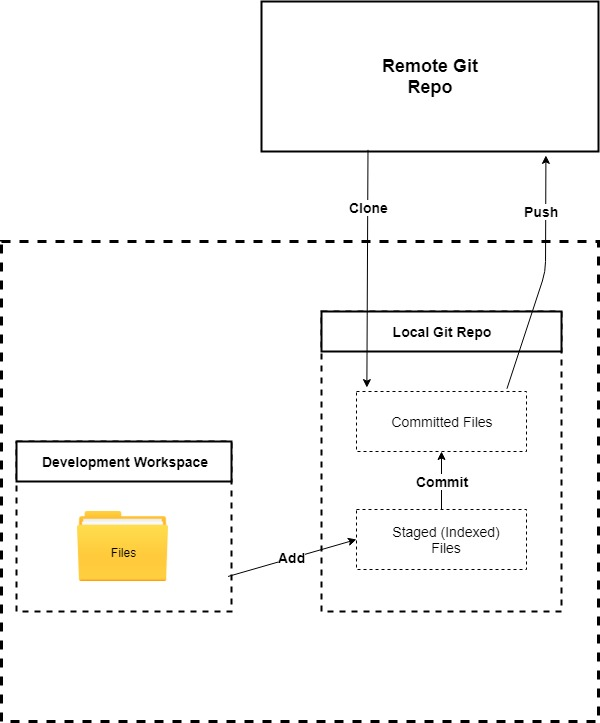
\includegraphics[width=14cm, height=14cm]{Git-Konzept.jpg}
		\caption{Git-Konzepte} 
		\label{ Git-Konzepte} 
	\end{center}
\end{figure}
Nun wird erklärt, wie das oben Genannte Git-Konzepte in diesem Fall angewendet wird. 
\newline
Um Git aus einem Java-Programm zu verwenden, gibt es eine voll funktionsfähige Git-Bibliothek namens JGit. JGit ist eine relativ vollständige Implementierung von Git, die ursprünglich in Java geschrieben wurde und in der Java-Community weit verbreitet ist.
Es gibt verschiedene Möglichkeiten, ein Projekt mit JGit zu verbinden und Code dagegen zu schreiben. Am einfachsten ist wahrscheinlich die Verwendung von Maven - die Integration erfolgt durch Hinzufügen des folgenden Snippets zum <dependencies>Tag in der pom.xml-Datei:
\begin{lstlisting}[language=XML,caption=JGit-dependency ]
<dependency>
<groupId>org.eclipse.jgit</groupId>
<artifactId>org.eclipse.jgit</artifactId>
<version>3.5.0.201409260305-r</version>
</dependency>
\end{lstlisting} 
Angenommen, der Administrator hat ein Remote-Git-Repository für ein bestimmtes Aufgabenblatt erstellt. Aus diesem Remote-Repository wird durch Git.cloneRepository () ein lokales Repository gemacht.
\begin{lstlisting}[language=JAVA,caption=clone Repository ]
public static Git cloneRepo(String repositoryUrl, String gitLocalRepositoryPath, String tfsUser, String password) throws GitAPIException, IOException {
   Path path = Paths.get(gitLocalRepositoryPath);
  if (!Files.exists(path)) {
  CloneCommand cloneCommand = Git.cloneRepository().setURI(repositoryUrl).setDirectory(new File(gitLocalRepositoryPath));
  UsernamePasswordCredentialsProvider user = new UsernamePasswordCredentialsProvider(tfsUser, password);
  cloneCommand.setCredentialsProvider(user);
  Git repository = cloneCommand.call();
  return repository;
  }else{Git repository = Git.open(new File(gitLocalRepositoryPath));
   System.out.println("exist" + repository.toString());

  return repository;
}
}
\end{lstlisting} 
Dieses lokale Repository wird sich in einem BackEnd-Ordner namens 'aufgabenblaetter' befindet. Die zum Ausführen des Tests erforderlichen Dateien werden nach dem Upload in diesem BackEnd-Ordner in seinem eigenen lokalen Repository gespeichert. Wenn beispielsweise Dateien zum Test von Aufgabenblatt-1 hochgeladen werden, werden sie unter 'aufgabenblaetter/Aufgabenblatt-1' gespeichert.
\newline
Jetzt erfolgt der Versand (Push) von Dateien vom lokalen Repository zum Remote-Repository. Wie bereits erwähnt, besteht dieser Prozess aus drei Schritten. Zunächst werden die Änderungen mit der von der Git-Bibliothek bereitgestellten add-Methode zum Staging-Bereich hinzugefügt.
\begin{lstlisting}[language=JAVA,caption=Add File To Index ]
public static boolean addFileToIndex(Git repository) throws IOException, GitAPIException {
try {
repository.add().addFilepattern(".").call();
return true;
} catch (Exception e) {
System.out.println(e.getMessage());
}
return false;
}
\end{lstlisting} 
Zweitens wird ein neues Commit mit dem aktuellen Inhalt des Index erstellt.
\begin{lstlisting}[language=JAVA,caption=commit Changes ]
	public static boolean commitChanges(Git repository, String commitMessage) throws GitAPIException, IOException {
repository.commit()
.setAll(true)
.setMessage("Commit changes to all files")
.call();

System.out.println("Committed all changes to repository at ");
return true;
}
\end{lstlisting} 
Drittens werden Commits vom lokalen Repository an das Remote-Repository übertragen.
\begin{lstlisting}[language=JAVA,caption=Push Changes ]
public static boolean pushChanges(Git repository) throws GitAPIException, URISyntaxException, IOException {
try
{
PushCommand pushCommand = repository.push();
pushCommand.setCredentialsProvider(new UsernamePasswordCredentialsProvider("swissi", "Mh123456"));
pushCommand.call();
return true;
}
catch (GitAPIException e)
{
throw new RuntimeException(e);
}
}
\end{lstlisting} 

 
\paragraph{Die zum Ausführen des Tests erforderlichen Dateien}
Jedes Git-Repository, das die Quellcodeverwaltung für ein bestimmtes Aufgabenblatt in der Remote-Testumgebung darstellt, hat die folgende Form und als Beispiel den folgenden Inhalt.
\newline
\dirtree{%
	.1 Aufgabenblatt-N.
	.2 makefile.
	.2 Jenkinsfile.
	.2 src.
	.3 ulam.c .
	.2 test.
	.3 ppr-tb-test-ulam.c.
}

Jedes Repository, unabhängig davon, welchem Aufgabenblatt es zugewiesen ist, enthält immer ein Makefile, ein Jenkinsfile, einen src-Ordner und einen test-Ordner.
\begin{itemize}
    \item \textbf{Src-Ordner: } Dies ist der unter-Repository-Ordner, in den der Student seine Aufgabenblattlösung hochladen wird. Dieser Vorgang wird nachstehend ausführlich erörtert.
	\item \textbf{Test-Ordner: } Hier wird die Datei mit den Testfällen vom Administrator hochgeladen.
	\item \textbf{Makefile: }  Wie bereits erwähnt, gibt es eine vom Administrator hochgeladene Testdatei und eine andere vom Studenten hochgeladene Lösungsdatei. Dies bedeutet, dass mehrere Quelldateien kompiliert werden müssen, um das Projekt zu bauen und ein Testergebnis zu erhalten. Um diesen Prozess zu erleichtern und solches Hindernis zu überwinden wird in diesem Fall ein Makefile benutzt.
	\newline
	Ein Makefile wird mit dem UNIX-Dienstprogramm 'make' verwendet, um zu bestimmen, welche Teile eines Programms kompiliert werden sollen. Ein Makefile ist im Grunde ein Skript, mit dem das Dienstprogramm make die geeigneten Programmdateien auswählt, die kompiliert und miteinander verknüpft werden sollen. Das Dienstprogramm make protokolliert die letzten Aktualisierungen von Dateien, sodass nur die Dateien aktualisiert werden, die Änderungen enthalten. Es müssen jedoch auch alle Dateien kompiliert werden, die von den aktualisierten Dateien abhängig sind, was sehr zeitaufwändig sein kann. Mit Hilfe von makefile automatisiert das Dienstprogramm make diese Kompilierung, um sicherzustellen, dass alle aktualisierten Dateien - und nur diese - kompiliert werden und dass die neuesten Versionen der Dateien mit dem Hauptprogramm verknüpft sind.
	\newline
	Ein Makefile enthält drei Arten von Informationen für das make-Programm: ein Ziel oder auch target genannt wird, das normalerweise der Name einer Datei, die von einem Programm generiert wird. Beispiele ausführbare Dateien oder Objektdateien. Es enthält auch Abhängigkeiten und Regeln (Befehle), die angeben, wie das Ziel aus den Quellen erstellt werden soll. 
	 
	\item \textbf{Jenkinsfile: } Ist eine Textdatei, die die Definition einer Jenkins-Pipeline enthält und in die Quellcodeverwaltung eingecheckt wird. Die Rolle dieser Datei wird nachfolgend erläutert.
	\end{itemize}
Bevor zu den folgenden Abschnitten übergangen wird, wird erläutert,wie der Student seine Lösungsdatei hochladen kann.
\paragraph{Student-Lösungsdatei hochladen}
Der Student lädt die zu testende Datei über die Frontend-Seite. Er wählt die Datei aus und drückt dann die Upload-Taste. Das Backend erhält also eine Anfrage zum Hochladen von Dateien. Um diese Aufgabe auszuführen, muss das BackEnd die folgenden Schritte ausführen: Angenommen, der Benutzer möchte seine Aufgabenblatt-1-Lösung zum ersten Mal testen. Anschließend wird aus dem lokalen Git-Repository von Aufgabenblatt-1 ein Branch mit dem Benutzernamen als Namen erstellt. Dann wird Die Datei durch Ausführen der Methoden Jgit-add und -commit an den angegebenen Branch gesendet. Der Benutzer hat nun die Möglichkeit, entweder den Test abzubrechen, was bedeutet, dass die hochgeladene Datei gelöscht wird, oder fortzufahren und den Testknopf zu drücken. Angenommen, der Benutzer hat den Test abgeschlossen und die Testtaste gedrückt. Dann wird der Student-Branch durch eine Jgit-Push-Methode an das Remote-Repository übertragen. Zur weiteren Verdeutlichung wird eine grafische Darstellung angezeigt, die diesen Vorgang erläutert.
\begin{figure}[h!]
	\begin{center}
		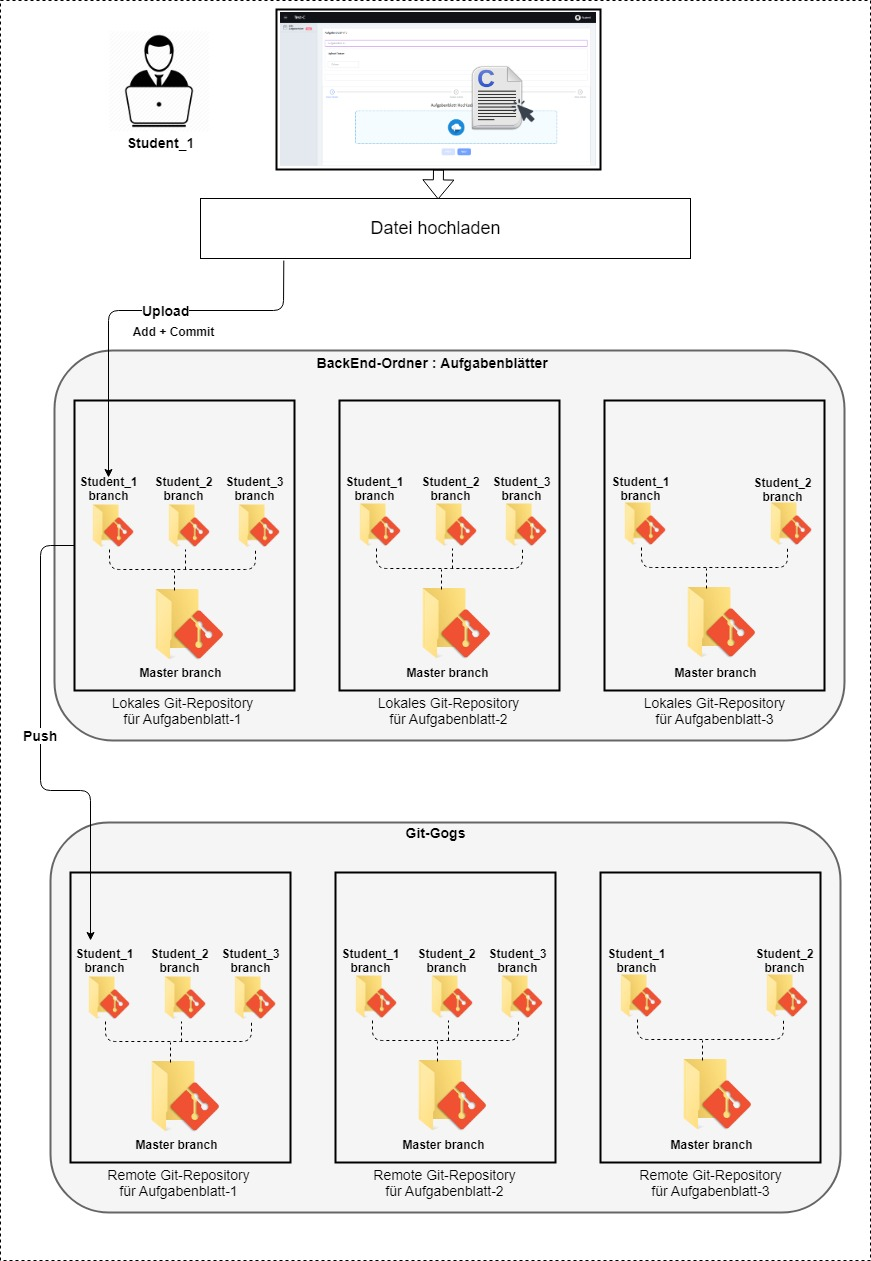
\includegraphics[width=15cm, height=17cm]{Loesungupload.jpg}
		\caption{Hochladen von Lösungsdatei} 
		\label{ Hochladen von Lösungsdatei } 
	\end{center}
\end{figure}

Für jedes Aufgabenblatt wird ein lokales und ein remote Git-Repository erstellt. Für jeden Student wird aus jedem Aufgabenblatt-Repository ein Branch erzeugt. 
\newline
Es wird beispielsweise davon ausgegangen, dass der Administrator drei Aufgabenblätter hinzufügt. Das heißt, es werden drei Git-Repositorys erstellt, von denen jedes ein Arbeitsblatt darstellt. Drei Studenten möchten ihre Lösungen testen. Zwei von ihnen haben die drei Übungsblätter gelöst und einer hat nur das erste und das zweite Aufgabenblatt gelöst. Anschließend werden aus den für die Aufgabenblätter 1 und 2 erzeugten Git-Repositorys drei Branchs erstellt. Weil die drei Studenten die ersten beiden Übungsblätter gelöst und getestet haben. Aus dem dritten Repositroy werden jedoch nur zwei Branchs erzeugt, da nur zwei Studenten ihre Aufgabenblatt-3-Lösung getestet haben.
\newline
Nun wird besprochen, wie nach Erhalt der Lösungsdatei der Test Prossez automatisch gestartet und das Ergebnis dem Student angezeigt wird.

\paragraph{Test Starten (jenkins Job Build)}
Wie bereits erwähnt, wird für jedes Repository automatisch ein Jenkins-Multibranch-Pipeline-Projekt generiert. Ein Multibranch-Pipeline-Projekt durchsucht einfach das Quellcode-Repository und erstellt automatisch einen Pipeline-Job für jedes Branch, das eine Jenkinsfile-Datei enthält. 
\newline
Eine Jenkinsfile-Datei ist eine Textdatei, die die Pipeline als Code enthält, der den gesamten Job-Workflow festschreibt. Daher lädt der Administrator diese Datei bei jeder Erstellung eines neuen Aufgabenblatts hoch. Dieser Vorgang ist in der folgenden Grafik dargestellt.
\begin{figure}[h!]
	\begin{center}
		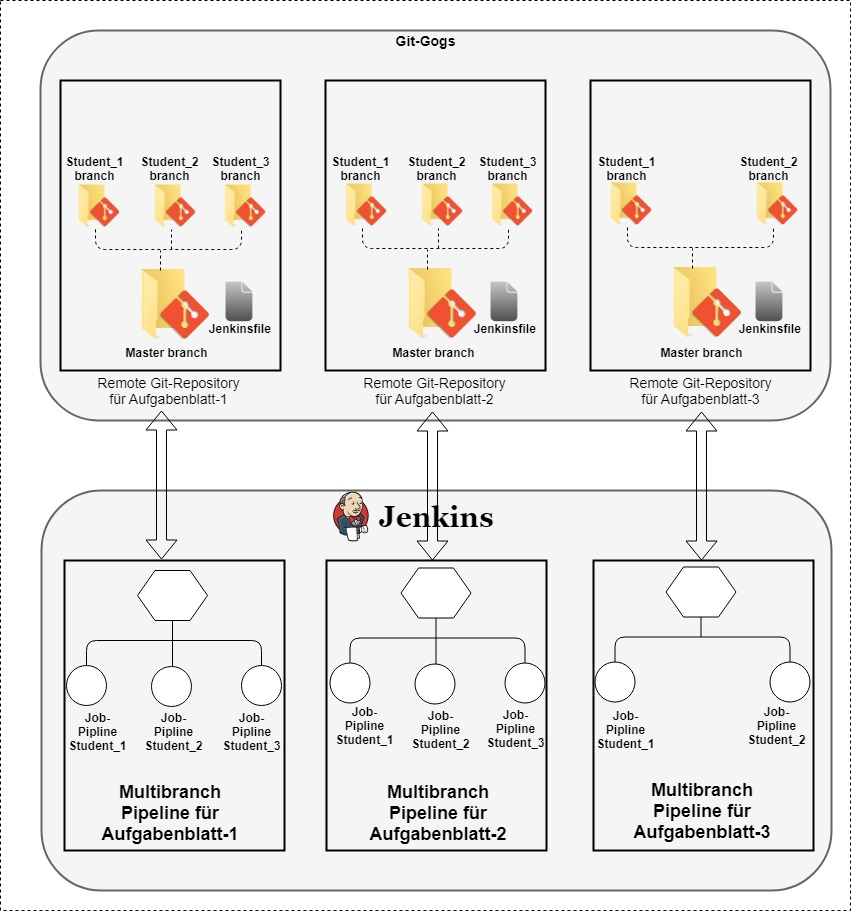
\includegraphics[width=13cm, height=14cm]{GogsJenkins.jpg}
		\caption{Multibranch Pipeline Projekt} 
		\label{ Multibranch Pipeline Projek } 
	\end{center}
\end{figure}
\newline
In diesem Fall besteht die Job-Pipeline nur aus einer Phase (stage), in der das Makefile ausgeführt werden sollte, um den Testprozess zu starten. Genau das, was in der Jenkinsfile-Datei steht.
\begin{lstlisting}[language=JAVA,caption=Jenkinsfile (Job-Pipeline-Skript) ]
pipeline{
agent any
stages {   
   stage ('Test with make file') {
       steps {
         sh 'make'
             }
                                 }
       }
      }
\end{lstlisting} 
'make' ist der Befehl zum Ausführen von makefile.
\newline
Jetzt werden sich die Ideen neu gruppieren und klar aufbauen. Der 'Student-1' hat die zu testende Datei hochgeladen. Zum Beispiel die Lösung von Übungsblatt-1. Wenn er seine Aufgabenblattlösung zum ersten Mal testet. Ein Branch namens 'Student-1' wird vom Aufgabenblatt-1-Repository erzeugt .Dann wird die Datei an diesem Branch übergeben. Wenn dies nicht der Fall ist und eine Branch vorhanden ist, wird es einfach verwendet. Dann wird Student-1-Branch auf Remote verschoben. Danach sendet das BackEnd eine Job-Build Anfrage an den Jenkins-Server. 
\begin{lstlisting}[language=JAVA,caption=Job-Build Anfrage ]
	public int buildJob(String jobName) throws JenkinsException {
int buildNumber = 0;
try{
JenkinsServer jenkinsServer = new JenkinsServer(new URI(jenkinsUrl), jenkinsUser, jenkinsPassword);
Map<String, Job> jobs = jenkinsServer.getJobs();
JobWithDetails job = jobs.get(jobName).details();
buildNumber = job.getNextBuildNumber();
job.build(true);
}catch (Exception e){
throw new JenkinsException(e);
}
return buildNumber;
}
\end{lstlisting} 

\subsubsection{Interne Prozesse}
\subsection{Alternativen}
\subsection{Ablauf des Testverfahrens}
\subsection{Installationsanleitung}
\subsection{Verwendung}
\section{Zusammenfassung}
\listoffigures
\section{Quellcodeverzeichnis}
\section{Quellenverzeichnis}
\end{document}